\chapter{Einbindung von Graphen}
\label{cha:graph}

Um Bilder in Latex einzubinden es ist nur wichtig dass sie im richtigen Format und im richtigen Verzeichnis vorliegen. Unter dem Ordner `` Dokumentation'' f�r diese Vorlage ist der Unterordner `` images '' angelegt. In diesem Ordner liegen alle Bilder die in diesem Dokument enthalten sind. Da k�nnen auch alle Bilder angelegt werden die in der Arbeit aufgerufen werden sollen. Die Bilder sollen f�r diese Vorlage in .pdf oder .jpg vorliegen. Die Bilder k�nnen auch direkt im Hauptverzeichnis angelegt werden.
\\Anhand folgenden Beispiels werden die Befehle erl�utert die man braucht um ein Bild in diesem Kapitel hinzuzuf�gen. 

\paragraph{Beispiel}

Das Bild mit dem Namen `` blockschaltbild.pdf '', das im Unterordner `` images '' liegt, wird mit folgenden Befehlen aufgerufen,

 {\textbackslash begin\{figure\}[ht]}
\\	{\textbackslash centering}
\\		{\textbackslash includegraphics[width=0.66\textbackslash textwidth]\{images/blockschaltbild.pdf\}}
\\	{\textbackslash caption\{Beispiel: Blockschaltbild \cite{guo}}}
\\	{\textbackslash label\{fig:blockschaltbild\}}
\\ {\textbackslash end\{figure\}}


\begin{figure}[!ht]
	\centering
		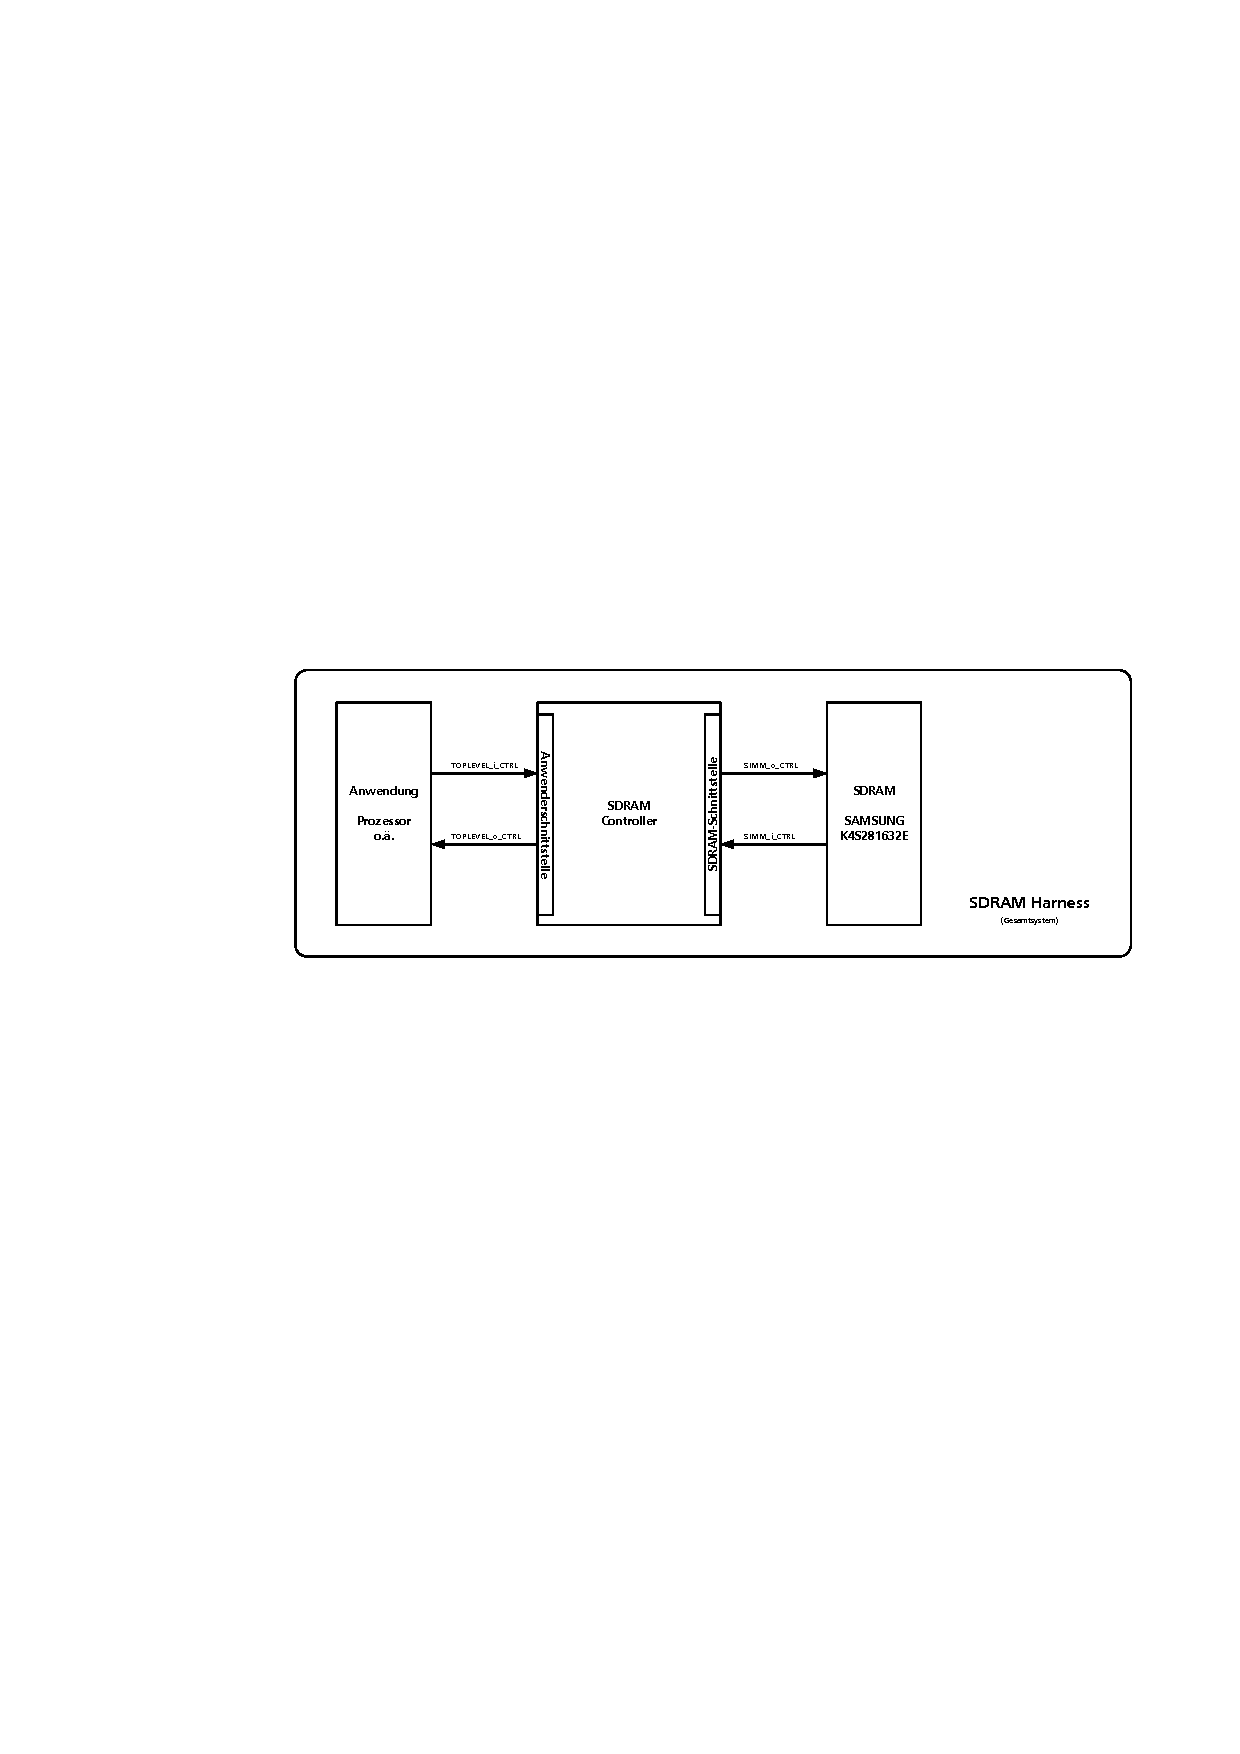
\includegraphics[width=0.66\textwidth]{images/blockschaltbild.pdf}
	\caption{Beispiel: Blockschaltbild \cite{guo}}
	\label{fig:blockschaltbild}
\end{figure}

%\begin{figure}[ht]
%	\centering
%		\includegraphics[width=1.00\textwidth]{images/busy-konflikt.jpg}
%	\caption{Busy-Konflikt im Einzelzugriff.}
%	\label{fig:busy-konflikt}
%\end{figure}
